\documentclass{swfubeamer}

\title{基于Linux的操作系统研究}

\author{CynYang}

\begin{document}

\frame{\titlepage}

\begin{frame}{总体设计框架}
  \begin{itemize}
  \item 启动模块
  \item 进程模块
  \item 内存模块
  \item 外围功能模块
  \end{itemize}
\end{frame}

\begin{frame}{开发环境}
  \begin{itemize}
  \item<1-4> 宿主OS
  \item<2-4> 虚拟机
  \item<3-4> 编译器
  \item<4-4> 编缉器
  \end{itemize}
  \begin{tabular}[center]{|l|c|}\hline
  \uncover<1-4> {\textit{debian}} & \uncover<1-4> {Linux debian v6.1.0.7-amd64}\\
  \uncover<2-4> {\textit{bochs}}  & \uncover<2-4> {Bochs v2.6.9}\\
  \uncover<3-4> {\bf nasm}        & \uncover<3-4> {Nasm v2.16.01}\\
  \uncover<3-4> {\bf gcc}         & \uncover<3-4> {Gcc v12.2.0}\\
  \uncover<4-4> {\textit{Emacs}}  & \uncover<4-4> {\small{GNU Emacs v28.2}}\\\hline
  \uncover<4-4> {\textit{Vim}}  & \uncover<4-4> {\small{GNU Vim v0.7.2}}\\\hline
  \end{tabular}
\end{frame}

\begin{frame}{启动模块}
  \begin{center}
    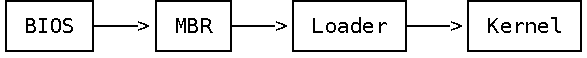
\includegraphics[width=.7\linewidth]{boot}
  \end{center}
\end{frame}

\begin{frame}{Mbr}
  \begin{itemize}
  \item \texttt{0x7C00}
  \item 512字节
  \item 加载Loader
  \end{itemize}
\end{frame}

\begin{frame}{实模式下的内存布局}
  \begin{center}
    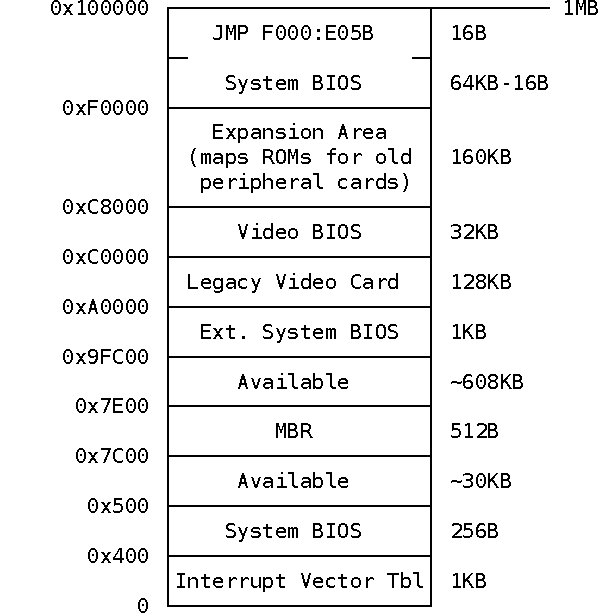
\includegraphics[width=.7\linewidth]{boot-mem}
  \end{center}
\end{frame}

\begin{frame}{Loader}
  \begin{itemize}
  \item 从实模式到保护模式
  \item 打开分页机制
  \item 加载Kernel
  \end{itemize}
\end{frame}

\begin{frame}{从实模式到保护模式}
  \begin{itemize}
  \item 把\texttt{0x92}第一个Bit置1
  \item 打开A20地址线
  \item 将CR0寄存器的PE Bit置1
  \end{itemize}
\end{frame}

\begin{frame}{分页机制}
  \begin{center}
    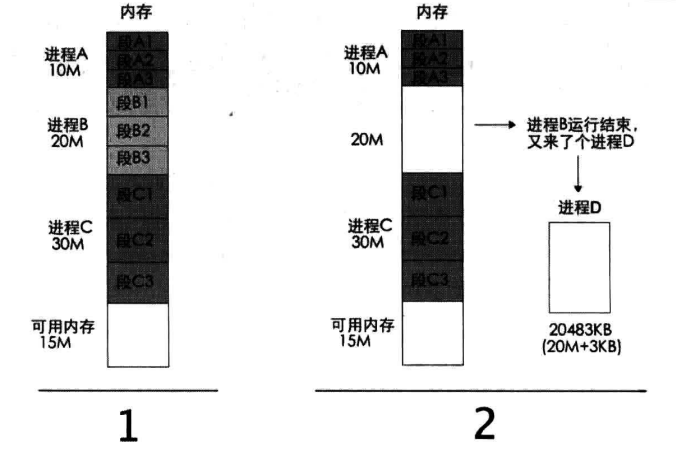
\includegraphics[width=.7\linewidth]{分页}
  \end{center}
\end{frame}

\begin{frame}{打开分页机制}
  \begin{itemize}
  \item 准备好页表目录和页表
  \item 将页表地址写入控制寄存器CR3
  \item 将寄存器CR0的PG Bit置1
  \end{itemize}
\end{frame}

\begin{frame}{加载Kernel}
  \begin{center}
    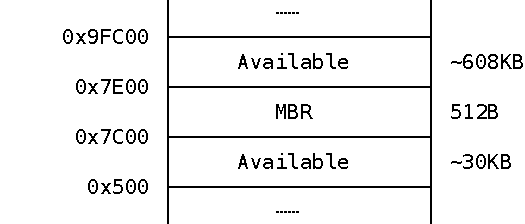
\includegraphics[width=.7\linewidth]{boot-mem2}
  \end{center}
\end{frame}

\begin{frame}{进程模块}
  \begin{itemize}
  \item 从特权级0到特权级3
  \item 创建用户进程
  \item 进程调度
  \end{itemize}
\end{frame}

\begin{frame}{内存模块}
  \begin{itemize}
  \item 初始化内存块描述符
  \item 分配/释放内存
  \end{itemize}
\end{frame}

\begin{frame}{外围功能模块}
  \begin{itemize}
  \item 文件系统
  \item Shell
  \end{itemize}
\end{frame}

\begin{frame}{文件系统}
  \begin{itemize}
  \item 创建文件
  \item 打开/关闭文件
  \item 写入/读取文件
  \item 删除文件
  \end{itemize}
\end{frame}

\begin{frame}{Shell}
  \begin{itemize}
  \item \Ctrl{L} 和 \Ctrl{U}
  \item ls
  \item cd
  \item mkdir
  \item rm
  \end{itemize}
\end{frame}

\end{document}

%%% Local Variables:
%%% mode: latex
%%% TeX-master: t
%%% TeX-master: "slides"
%%% TeX-master: t
%%% End:
